\documentclass [xcolor=svgnames, t] {beamer} 
\usepackage[utf8]{inputenc}
\usepackage{booktabs, comment} 
\usepackage[absolute, overlay]{textpos} 
\usepackage{pgfpages}
\usepackage[font=footnotesize]{caption}
\useoutertheme{infolines} 




\definecolor{brownbrown}{RGB}{56, 28, 0}
\definecolor{brownred}{RGB}{228, 0, 43}
\definecolor{myuniversity}{RGB}{56, 28, 0}

\setbeamercolor{title in head/foot}{bg=brownred, fg=brownbrown}
\setbeamercolor{author in head/foot}{bg=myuniversity}
\makeatletter
\setbeamertemplate{footline}{
  \leavevmode%
  \hbox{%
    \begin{beamercolorbox}[wd=\paperwidth,ht=2.25ex,dp=1ex,right]{date in head/foot}%
      \usebeamerfont{date in head/foot}
      \insertframenumber{} / \inserttotalframenumber\hspace*{2ex}
    \end{beamercolorbox}}%
  \vskip0pt%
}
\makeatother
\setbeamertemplate{page number in head/foot}{}
\usepackage{csquotes}


\usepackage{amsmath}
\usepackage[makeroom]{cancel}


\usepackage{textpos}

\usepackage{tikz}

\usetheme{Madrid}
\definecolor{myuniversity}{RGB}{56, 28, 0}
\usecolortheme[named=myuniversity]{structure}
\usepackage{tikz}



\title[RUNNING TITLE]{Dirty Access Tracking in GPU-UVM}
\author{\footnotesize Aditi Khandelia, Arush Upadhyaya, Kushagra Srivastava, Sankalp Mittal, Vidhi Jain\vspace{10mm}}

\institute[]{CS614 Course Project  \\Indian Institute of Technology, Kanpur}
\date{\today}


\addtobeamertemplate{navigation symbols}{}{%
    \usebeamerfont{footline}%
    \usebeamercolor[fg]{footline}%
    \hspace{1em}%
    \insertframenumber/\inserttotalframenumber
}



\begin{document}
\begin{frame}
\maketitle
\end{frame}


\begin{frame}
\frametitle{Table of Contents}
\tableofcontents
\end{frame}

\section{Introduction}
\begin{frame}{Introduction}
\begin{itemize}
    \item NVIDIA's \textbf{Unified Virtual Memory (UVM)} framework presents a shared address space to the CPU and GPU, servicing page residency via a hardware fault-driven migration mechanism
    \item The existing UVM implementation provides no facility to track \textit{which} virtual pages have been written by the GPU, nor the temporal ordering of such writes
    \item This work presents a \textbf{dirty page tracking} subsystem integrated directly into the UVM kernel module, offering:
    \begin{itemize}
        \item Instrumentation of the GPU write-fault servicing path to record per-page first-write timestamps
        \item Per-process isolation of tracking state via nested \texttt{xarray} structures indexed by PID
        \item A \texttt{procfs}-based query interface supporting address range filtering
    \end{itemize}
    \item The system enables precise post-hoc attribution of GPU memory writes
\end{itemize}
\end{frame}

\section{Motivation}
\begin{frame}{Motivation}
\begin{itemize}
    \item \textbf{Fault-tolerant training:} Large ML training jobs that crash must restart from scratch; knowing which model parameter pages were updated enables incremental checkpointing and reduces recovery time
    \item \textbf{GPU process live migration:} Migrating a running GPU process between nodes requires identifying dirty pages to minimise data transfer; no such mechanism exists in the UVM stack today
    \item \textbf{Memory overcommitment:} Operating systems swap CPU pages using dirty bits; an analogous mechanism for GPU memory requires kernel-level write tracking that hardware does not expose directly
    \item \textbf{Heterogeneous synchronisation:} In CPU-GPU workloads with alternating phases, only pages written by the GPU need to be synchronised back to the host
\end{itemize}
\end{frame}

\section{Methodology}
\begin{frame}{Implementation Idea}
\begin{itemize}
    \item GPU write faults are already handled by the UVM kernel module to migrate pages; this fault path is the natural point at which a write can be observed
    \item On each write fault, record the faulting page number and a kernel timestamp into a per-process data structure; subsequent writes to the same page are ignored
    \item Maintain one table per process, so that tracking for one process does not interfere with another
    \item Expose the accumulated dirty set to userspace via procfs, allowing any tool to query which pages were written and when without modifying the application
    \item Provide an explicit start/stop interface so that tracking is scoped to a region of interest, and a fresh table is guaranteed on each start
\end{itemize}
\end{frame}

\subsection{Data Structures}
\begin{frame}{Implementation: Data Structures}
\begin{itemize}
    \item Two nested \texttt{xarray} structures form the core of the tracking state:
    \begin{itemize}
        \item A global \texttt{xarray} maps each PID to a \texttt{uvm\_dirty\_page\_table} instance
        \item Each \texttt{uvm\_dirty\_page\_table} contains a second \texttt{xarray} mapping page numbers to \texttt{dirty\_page\_info} entries
    \end{itemize}
    \item Each \texttt{dirty\_page\_info} record stores the page number, a \texttt{ktime\_get\_ns()} timestamp captured at fault-service time (not at the write itself), and the PID
    \item \texttt{xarray} is used throughout for its lock-free read semantics and O(1) indexed lookup; allocations in the fault path use \texttt{GFP\_ATOMIC} to avoid sleeping in interrupt context
    \item First-write-wins semantics: if an entry already exists for a page, the record call is a no-op, preserving the earliest observed timestamp
\end{itemize}
\end{frame}

\subsection{Fault Hook}
\begin{frame}{Implementation: Fault Hook}
\begin{itemize}
%    \item A conditional is inserted into the GPU replayable fault handler in \texttt{uvm\_gpu\_replayable\_faults.c}; on a write fault, if tracking is active for the faulting PID, the page is recorded
%    \item \textbf{Invalidation on start:} When tracking is enabled, all existing GPU page table mappings for the process are invalidated, forcing fresh faults on subsequent accesses so that no write goes unobserved
%    \item This ensures that pages written before tracking was enabled but still resident in the GPU page table are not silently missed
	\item \textbf{Invalidation on start:} When tracking is enabled, all existing GPU page table mappings for the process are invalidated, forcing fresh faults on subsequent accesses so that no write goes unobserved.
	\item \textbf{On a write fault:} A conditional is inserted into the GPU replayable fault handler in \texttt{uvm\_gpu\_replayable\_faults.c}; if tracking is active for the faulting PID, the page address and timestamp are recorded in the dirty table before the mapping is restored and the instruction is replayed.
	\item \textbf{On a read fault:} A conditional is inserted into the VA block fault-servicing path in \texttt{uvm\_va\_block.c}; if tracking is active, the page is re-mapped read-only instead of read-write, ensuring that any subsequent write to that page still generates a fault and is recorded rather than completing silently through an already-valid mapping.
\end{itemize}
\end{frame}

\subsection{procfs Interface}
\begin{frame}{Implementation: procfs Interface}
Five entries are exposed under \texttt{/proc/driver/nvidia-uvm/}:
\begin{itemize}
    \item \texttt{dirty\_pids\_start\_track}: initialise a fresh dirty page table for the calling process and invalidate existing GPU mappings
    \item \texttt{dirty\_pids\_stop\_track}: destroy the table for the calling process and cease recording
    \item \texttt{dirty\_pid\_to\_query}: select which process's table is read on the next \texttt{dirty\_pages} access
    \item \texttt{dirty\_range}: set a virtual address range filter; only pages within the range are returned
    \item \texttt{dirty\_pages}: read out recorded entries as \texttt{(address, timestamp, pid)} tuples; reads are non-destructive
\end{itemize}
\end{frame}

\section{Testing and Evaluation}

\begin{frame}{Testing Mechanism}
\begin{itemize}
    \item All tests are CUDA C programs that interact with the tracking subsystem exclusively via the procfs interface; no modifications to application or kernel source are required per test
    \item Tests require root access and use \texttt{cudaMallocManaged} for UVM allocations
    \item The test suite is organised into three correctness categories:
    \begin{itemize}
        \item \textbf{Table lifecycle:} init, destroy, and reinit behaviour; multi-region and stress scenarios
        \item \textbf{Ordering:} write-before-start exclusion, timestamp monotonicity, non-destructive reads, first-write-wins under concurrent streams
        \item \textbf{Address range filtering:} range isolation, subpage alignment, inverted and zero-length ranges, concurrent range-read races
    \end{itemize}
    \item Performance is evaluated separately via five microbenchmarks covering write overhead, duplicate fault cost, contention, table lifecycle cost, and per-fault recording cost
\end{itemize}
\end{frame}

\begin{frame}{Performance Analysis: Write Overhead}
\begin{block}{}
\scriptsize Measures kernel execution time and percentage overhead for a pure-write workload with tracking on vs.\ off, across varying allocation sizes.
\end{block}
\begin{columns}
    \column{0.5\textwidth}
    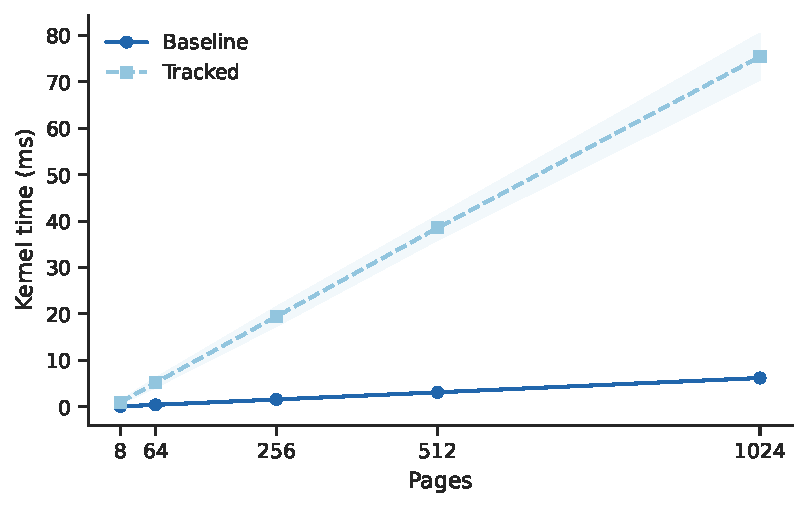
\includegraphics[width=\linewidth]{figures/tc01_time_vs_pages.pdf}\\
    {\scriptsize Both curves scale linearly; the tracked curve is ${\approx}12\times$ higher, reflecting per-page fault-servicing cost.}
    \column{0.5\textwidth}
    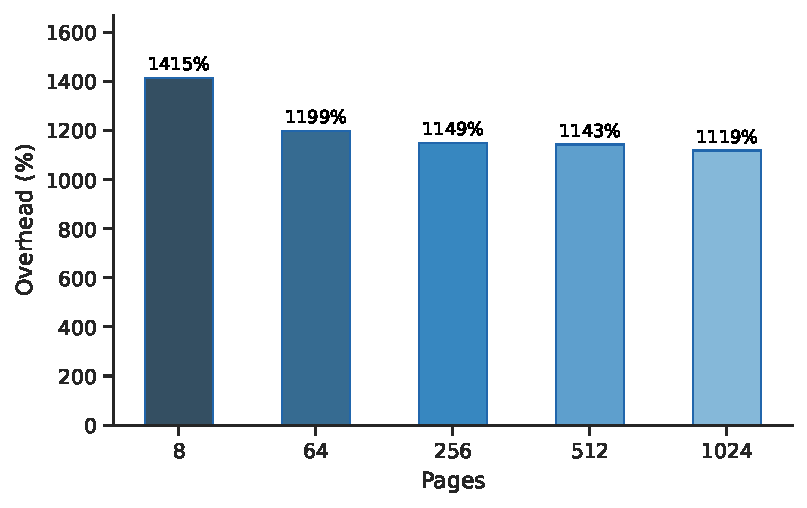
\includegraphics[width=\linewidth]{figures/tc01_overhead_vs_pages.pdf}\\
    {\scriptsize Overhead peaks at $1725\%$ for small allocations where fixed invalidation cost dominates, converging to $1090$--$1160\%$ at scale.}
\end{columns}
\end{frame}

\begin{frame}{Performance Analysis: Workload Breakdown}
\begin{block}{}
\scriptsize Benchmarks READ, WRITE, and MIXED workloads across five page counts with tracking on and off, averaged over 10, 50, and 200 iterations.
\end{block}
\begin{columns}
    \column{0.5\textwidth}
    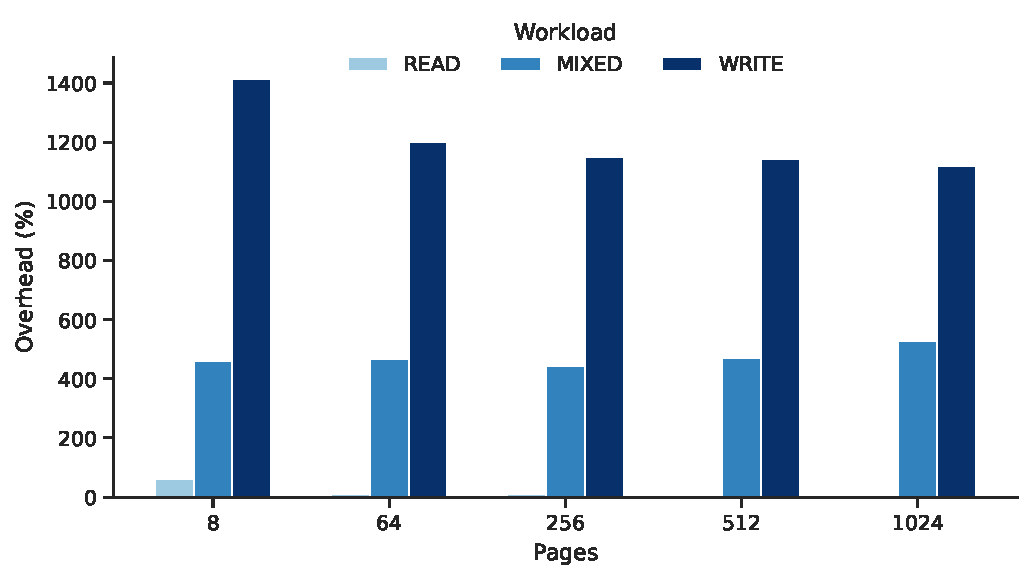
\includegraphics[width=\linewidth]{figures/tc02_overhead_grouped.pdf}\\
    {\scriptsize READ: $6$--$95\%$; MIXED: $415$--$497\%$; WRITE: $1090$--$1725\%$. Overhead is strictly proportional to write-faulting pages.}
    \column{0.5\textwidth}
    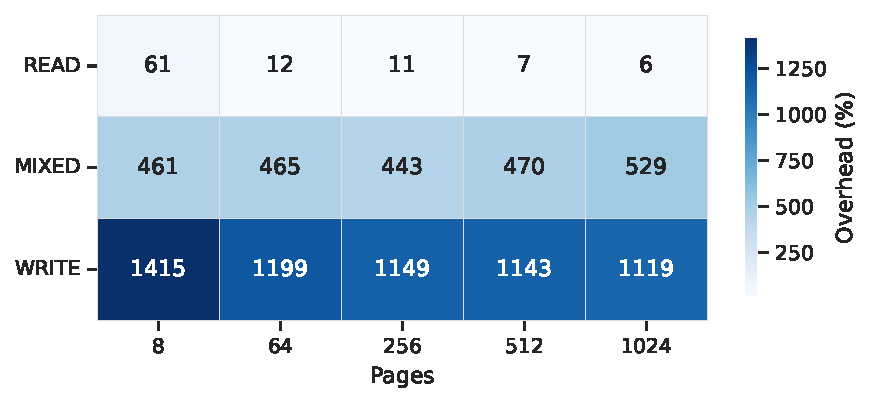
\includegraphics[width=\linewidth]{figures/tc02_overhead_heatmap.pdf}\\
    {\scriptsize Heatmap confirms the trend; READ rows are uniformly cool, WRITE rows uniformly hot across all page counts.}
\end{columns}
\end{frame}

\begin{frame}{Performance Analysis: Single Fault Recording Cost}
\begin{block}{}
\scriptsize Isolates the per-fault recording overhead using a single-thread kernel writing 4096 pages serially, run 100 times with and without tracking.
\end{block}
\begin{columns}
    \column{0.5\textwidth}
    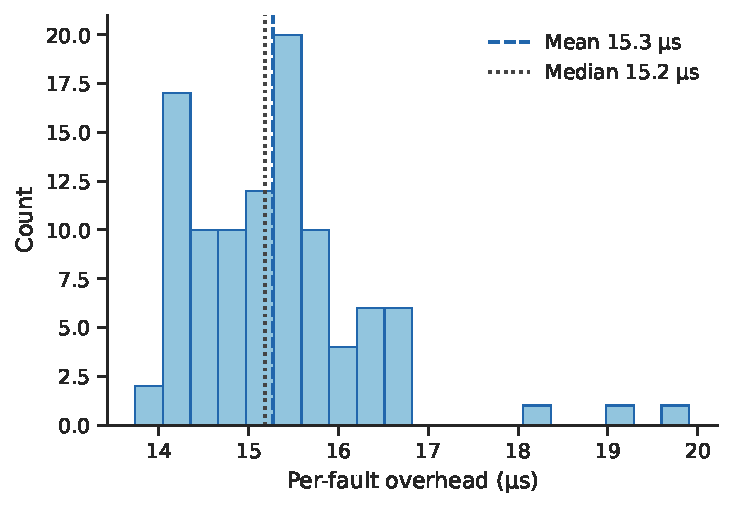
\includegraphics[width=\linewidth]{figures/single_fault_overhead_hist.pdf}\\
    {\scriptsize Per-fault overhead concentrated around ${\approx}15.3\,\mu$s mean, indicating a stable and predictable per-page recording cost.}
    \column{0.5\textwidth}
    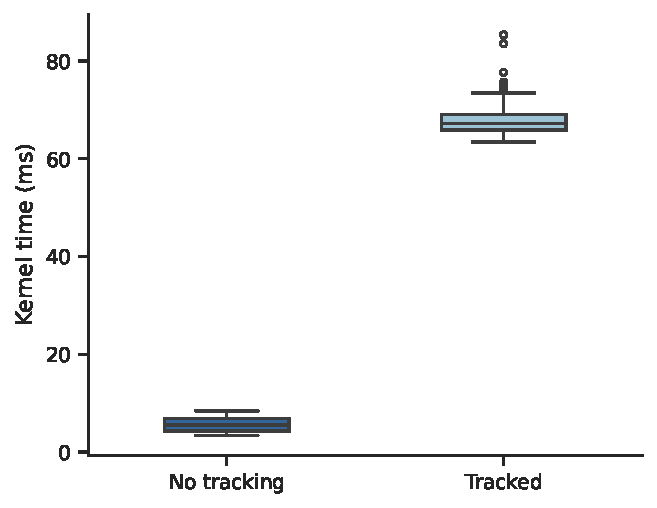
\includegraphics[width=\linewidth]{figures/single_fault_boxplot.pdf}\\
    {\scriptsize Boxplot confirms low variance across runs; the recording path behaves consistently with minimal outliers.}
\end{columns}
\end{frame}

\begin{frame}{Performance Analysis: Duplicate Fault Skip Cost}
\begin{block}{}
\scriptsize Measures the cost of the first-write-wins skip path by writing the same pages twice within one epoch. Quantifies whether the xarray lookup on a duplicate fault is cheaper than a full insertion.
\end{block}
\begin{columns}
    \column{0.5\textwidth}
    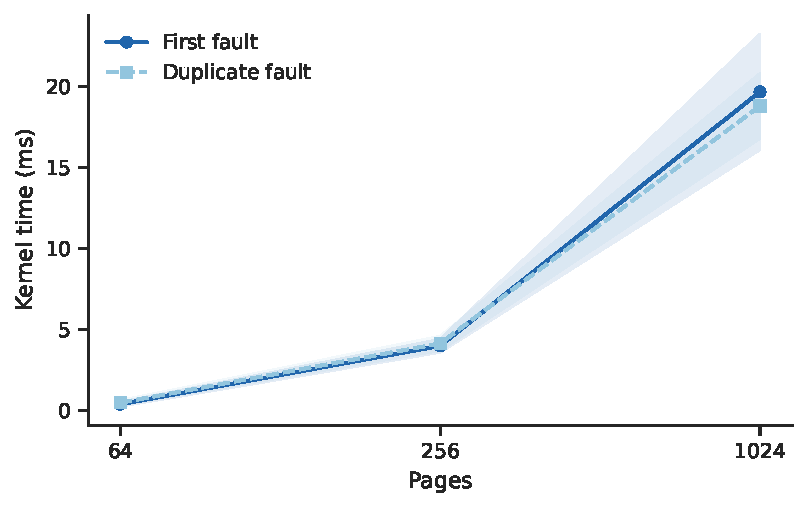
\includegraphics[width=\linewidth]{figures/dup_fault_time_vs_pages.pdf}\\
    {\scriptsize First and duplicate fault times track each other closely; the skip path offers little savings.}
    \column{0.5\textwidth}
    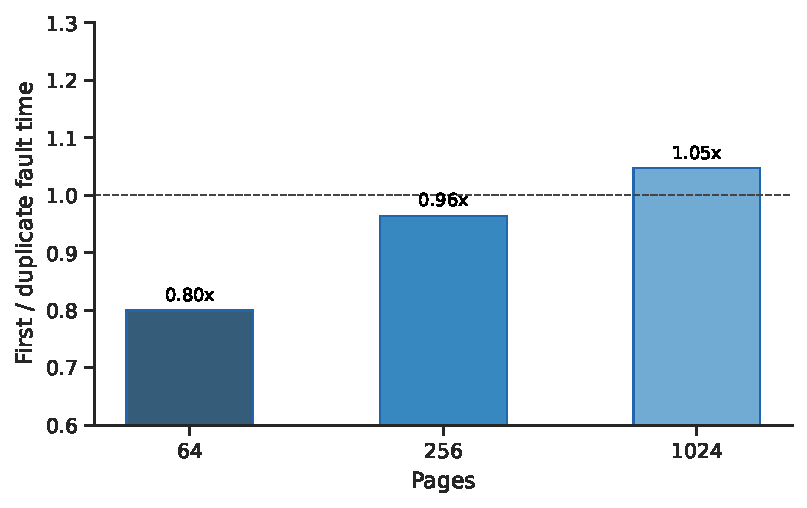
\includegraphics[width=\linewidth]{figures/dup_fault_ratio_vs_pages.pdf}\\
    {\scriptsize Ratio near $1.0$ indicates the bottleneck is fault-servicing itself, not the xarray insertion.}
\end{columns}
\end{frame}

\begin{frame}{Performance Analysis: Contention}
\begin{block}{}
\scriptsize Runs multiple CUDA streams concurrently under disjoint (each stream writes separate pages) and hot-set (all streams write the same pages) conditions.
\end{block}
\begin{columns}
    \column{0.5\textwidth}
    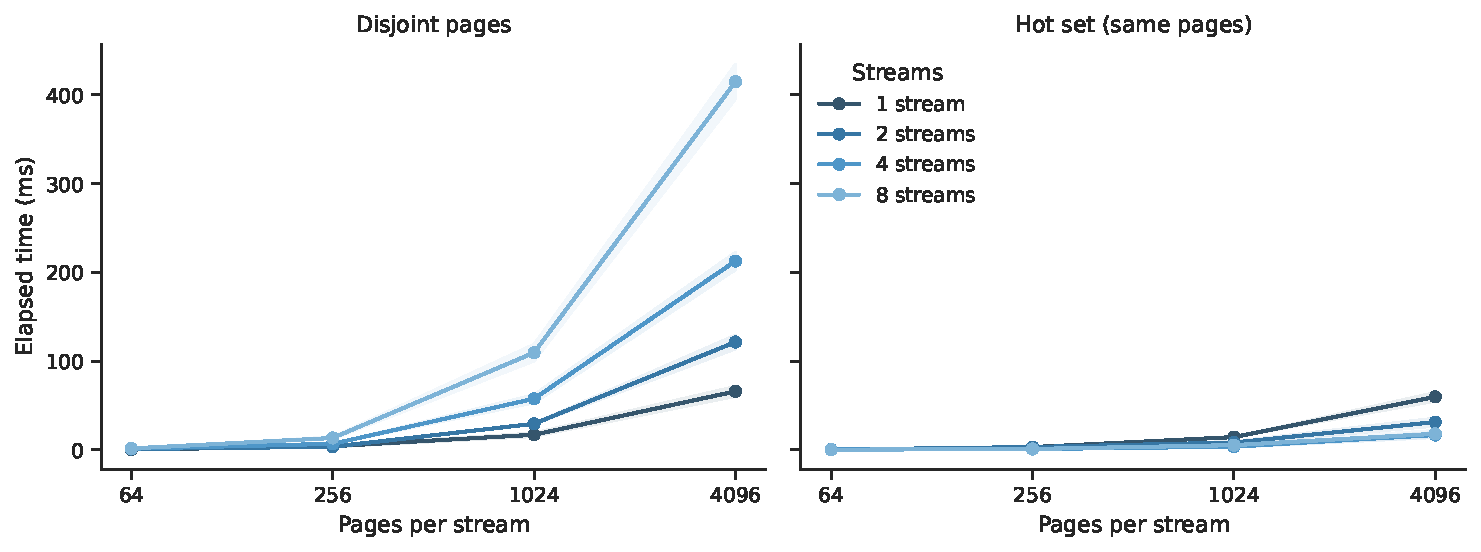
\includegraphics[width=\linewidth]{figures/contention_time_vs_pages.pdf}\\
    {\scriptsize Hot-set elapsed times are consistently lower; concurrent streams hitting already-recorded pages trigger the skip path, reducing total work.}
    \column{0.5\textwidth}
    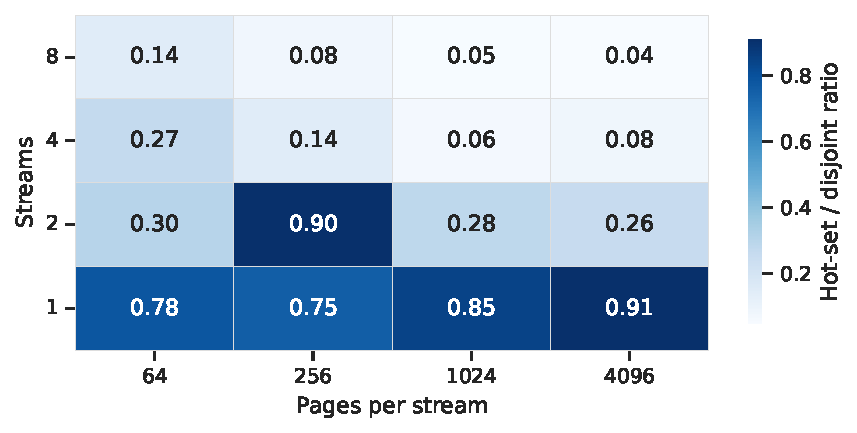
\includegraphics[width=\linewidth]{figures/contention_ratio_heatmap.pdf}\\
    {\scriptsize Hot-set advantage grows with stream count as skip-path hits increase.}
\end{columns}
\end{frame}

\begin{frame}{Performance Analysis: Table Lifecycle Cost}
\begin{block}{}
\scriptsize Times the three procfs lifecycle operations: init (allocates empty xarray, invalidates GPU PTEs), destroy (frees all recorded entries), and reinit (destroy followed by re-invalidation).
\end{block}
\begin{columns}
    \column{0.5\textwidth}
    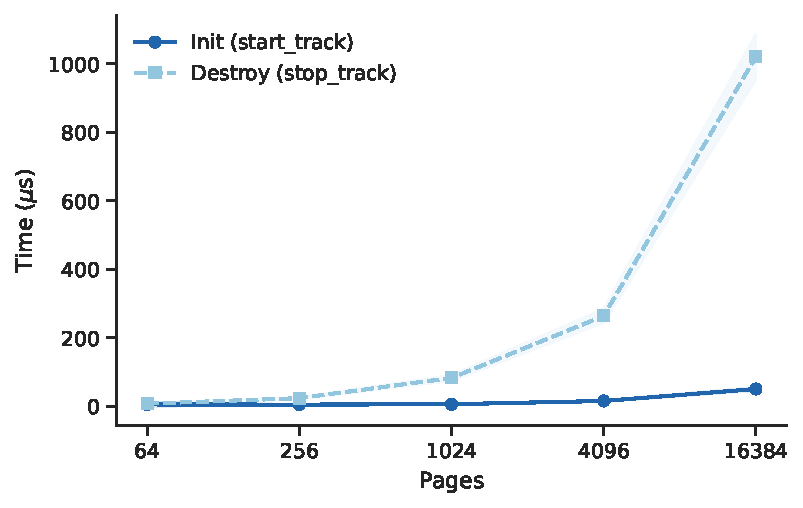
\includegraphics[width=\linewidth]{figures/lifecycle_init_destroy.pdf}\\
    {\scriptsize Init is nearly flat at $5$--$51\,\mu$s ($O(1)$ xarray allocation); destroy scales linearly to ${\approx}1\,\mathrm{ms}$ at 16384 pages.}
    \column{0.5\textwidth}
    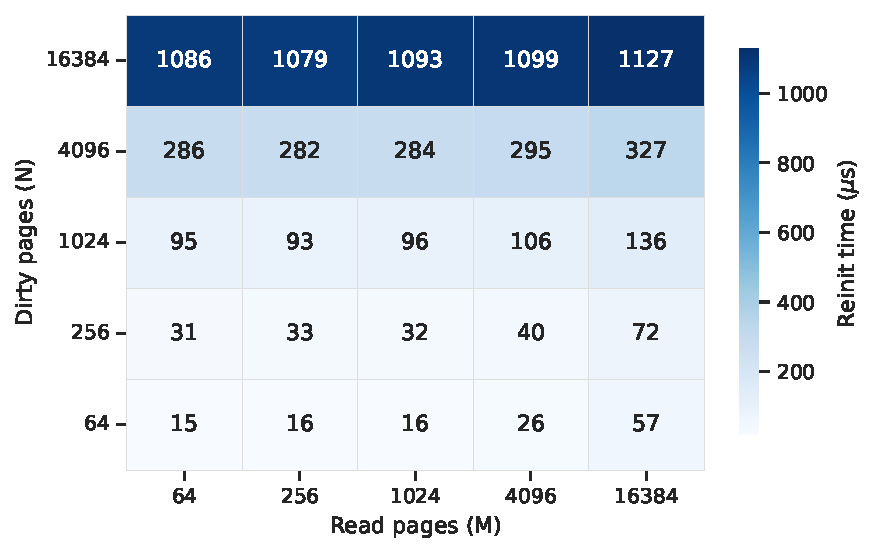
\includegraphics[width=\linewidth]{figures/lifecycle_reinit_heatmap.pdf}\\
    {\scriptsize Reinit cost rises steeply with dirty pages ($N$) and gently with read pages ($M$), as destroy dominates over PTE invalidation.}
\end{columns}
\end{frame}

\section{Ongoing Work and Next Steps}

\begin{frame}{Ongoing Work: Profiling and Analysis}
\begin{itemize}
    \item \textbf{Function-specific profiling:} Insert \texttt{ktime} probes at entry and exit of individual UVM fault-handling functions to decompose total fault latency into per-function contributions
    \item \textbf{Deterministic profiling:} Current microbenchmarks show variance from GPU scheduling jitter; designing workloads with fixed, predictable access patterns to obtain stable measurements
    \item \textbf{Lock characterisation:} Instrumenting the range-filter spinlock and xarray internal locks to quantify contention under increasing stream counts and identify whether locks or fault-servicing dominate overhead
    \item \textbf{Memory footprint profiling:} Measuring per-entry xarray cost under large dirty sets; comparing against a bitmap representation to identify the crossover density at which a bitmap becomes more efficient
\end{itemize}
\end{frame}

\begin{frame}{Next Steps: Optimisations}
\begin{itemize}
    \item \textbf{Write-permission removal:} Revoke write permissions only rather than full PTE invalidation at epoch start, reducing overhead for non-tracked and read-only pages
    \item \textbf{Parallel invalidation:} Distribute \texttt{va\_block} invalidation across multiple kernel threads to make tracking onset more deterministic
    \item \textbf{Lockless recording:} Replace the coarse spinlock with per-entry locking or a fully lockless xarray path to reduce contention under high-concurrency workloads
    \item \textbf{Differential function priority:} Assign higher scheduling priority to fault-servicing functions on the critical path to reduce timing jitter
    \item \textbf{Bitmap representation:} For high-density dirty sets, replace the xarray with a bitmap to reduce memory overhead and improve read locality
\end{itemize}
\end{frame}

\begin{frame}{Next Steps: Extensions and Deliverables}
\begin{itemize}
    \item \textbf{Tracking status query:} Lightweight procfs entry to check whether tracking is active for a given PID
    \item \textbf{CPU-side dirty tracking:} Extend to CPU writes via \texttt{mmu\_notifier} integration, exposed through the existing procfs interface
    \item \textbf{Per-page write counters:} Track write frequency beyond first-write-wins to support migration and eviction decisions
\end{itemize}
\end{frame}

\section{Conclusion}

\begin{frame}{}
\vfill
\begin{center}
    {\Large \textbf{Thank You}}
\end{center}
\vfill
\end{frame}

\end{document}
